% $Id: perspectives.tex 12369 2010-09-28 08:34:59Z markus $
% Local Variables:
% ispell-check-comments: nil
% Local IspellDict: american
% End:
% --------------------------------------------------------
% User documentation
% copyright by BREDEX GmbH 2004
% --------------------------------------------------------
\subsection{The \specpersp{}}
\index{Specification!Perspective}
\index{Perspective!Specification}
\index{Browser!Test Suite}
\index{Browser!Test Case}
\index{Browser!Component Name}
\index{View!Editor}
\index{View!Properties}
\index{View!Data Sets}
\index{View!Problem}
\index{Test Suite!Browser}
\index{Test Case!Browser}
\index{Component Name Browser}
\index{Editor!View}
\index{Properties View}
\index{Data Sets View}
\index{Problem View}
\index{Component!Names!View}
\index{View!Component Names}
The \specpersp{} (\bxfigref{clientwindow}) provides browsers, editors and views to let you create and edit tests.

It contains:

\begin{itemize}
\item The \gdtestsuitebrowser{} 
\item The \gdtestcasebrowser{} 
\item The \gdcompnamebrowser{} 
\item The editor area 
\item The \gdpropview{} 
\item The \gddatasetsview{} 
\item The \gdcompnamesview{} 
\item The \gdprobview{} 
\item The search result view (behind the \gdprobview{})
\item The \gdrunautview{}
\end{itemize}

The \gdcompnamesview{}, \gddatasetsview{} and \gdpropview{} show you details about the currently selected item in the browser or editor. 

\begin{figure}
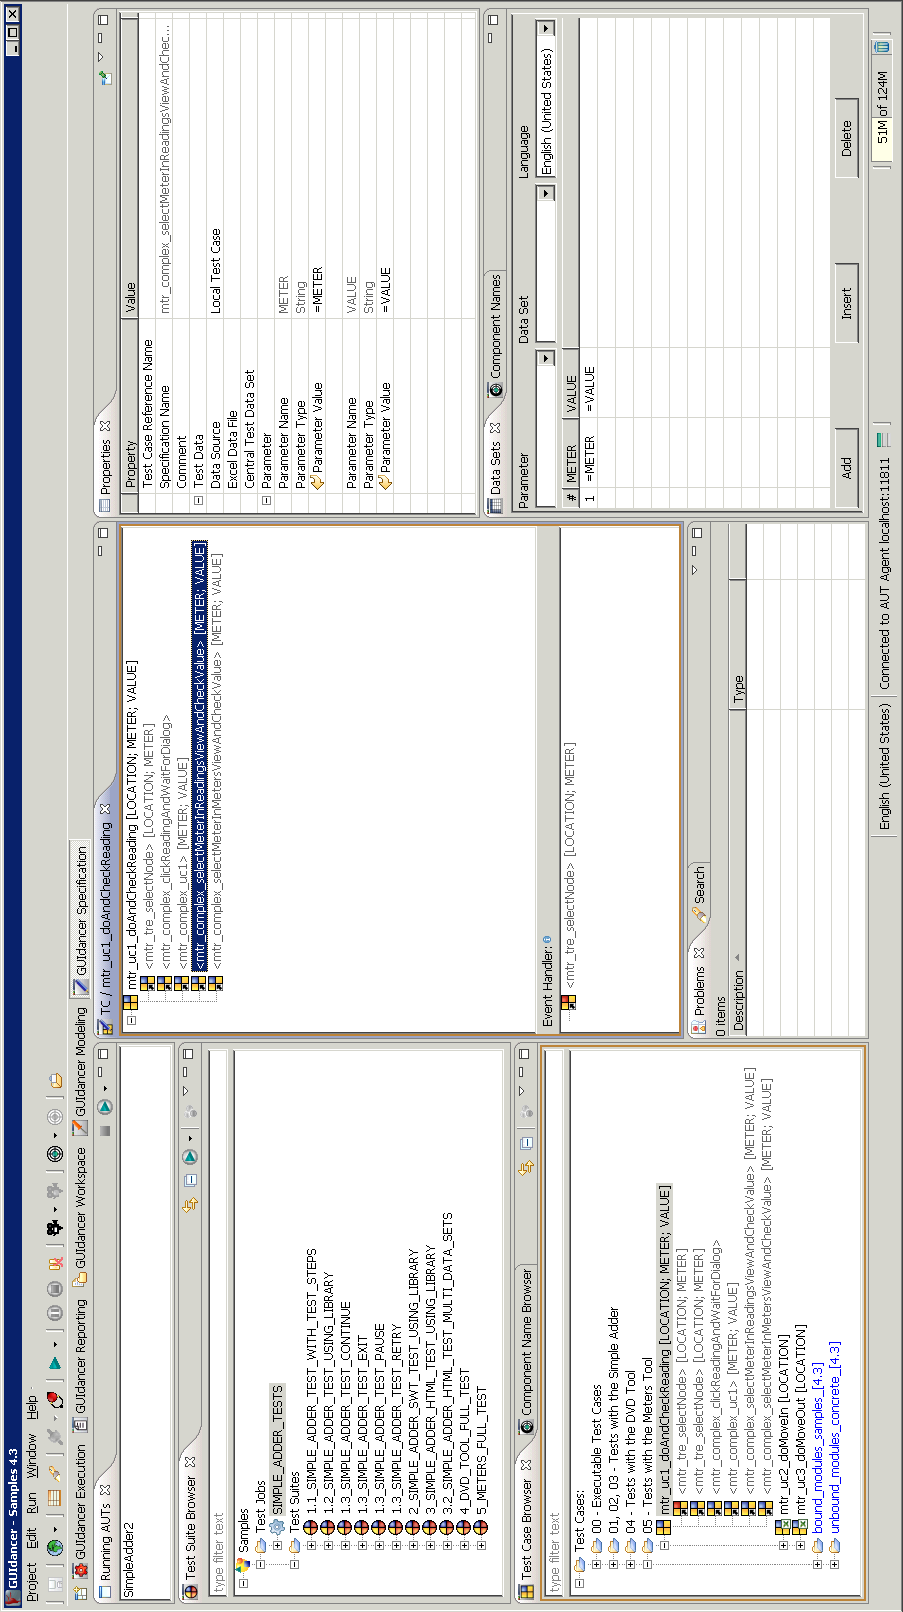
\includegraphics[width=12.5cm]{Userinterface/Editors/PS/client}
\caption{\app{} Specification Perspective}
\label{clientwindow}
\end{figure}


 \clearpage
\subsection{The \execpersp{}}
\index{Execution!Perspective}
\index{Perspective!Execution}
\index{Views!Test Result}
\index{Test Result!View}

In the \execpersp{}, you can see the following (\bxfigref{executionclient}):


\begin{itemize}
\item The \gdtestsuitebrowser{}
\item The \gdtestresultview{}
\item The \gdpropview{} 
\item The \gdimgview{}
\end{itemize}


\begin{figure}
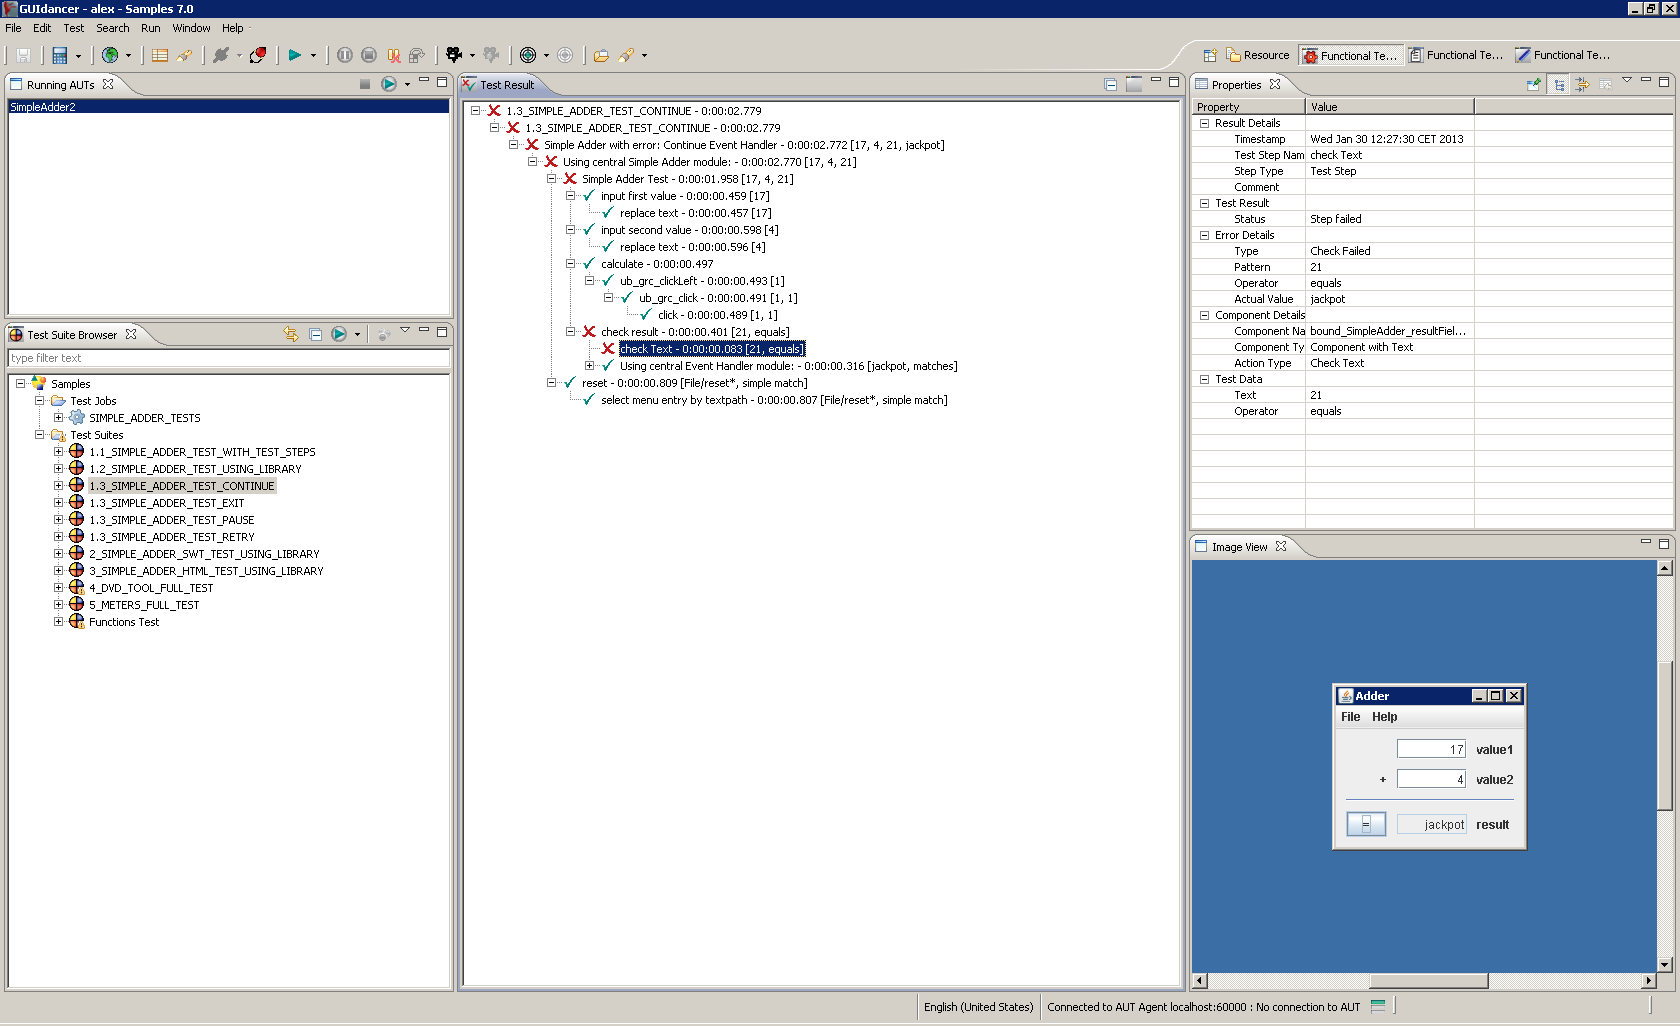
\includegraphics[width=12.5cm]{Userinterface/Editors/PS/executionclient}
\caption{\execpersp{}}
\label{executionclient}
\end{figure}

You cannot edit in the \execpersp{}, but you can see the results of tests that have been started interactively.. 
\clearpage

\subsection{The \reportpersp{}}
\index{Reporting!Perspective}
\index{Perspective!Reporting}
\index{Views!Test Result Summary}
\index{Test Result Summary!View}

In the \reportpersp{}, you can see an overview of all the test runs in the current \gddb{}, for all \gdprojects{} it contains. You can reopen test runs if the details for the report are still in the \gddb{} \bxpref{TasksReopenTestResult} and analyze the test using the \gdpropview{} and the \gdimgview{}. 

The \reportpersp{} (\bxfigref{reportingperspective}) contains the following views:

\begin{itemize}
\item The \gdtestresultview{}
\item The \gdpropview{} 
\item The \gdimgview{}
\item The \gdtestsummaryview{}
\end{itemize}


\begin{figure}
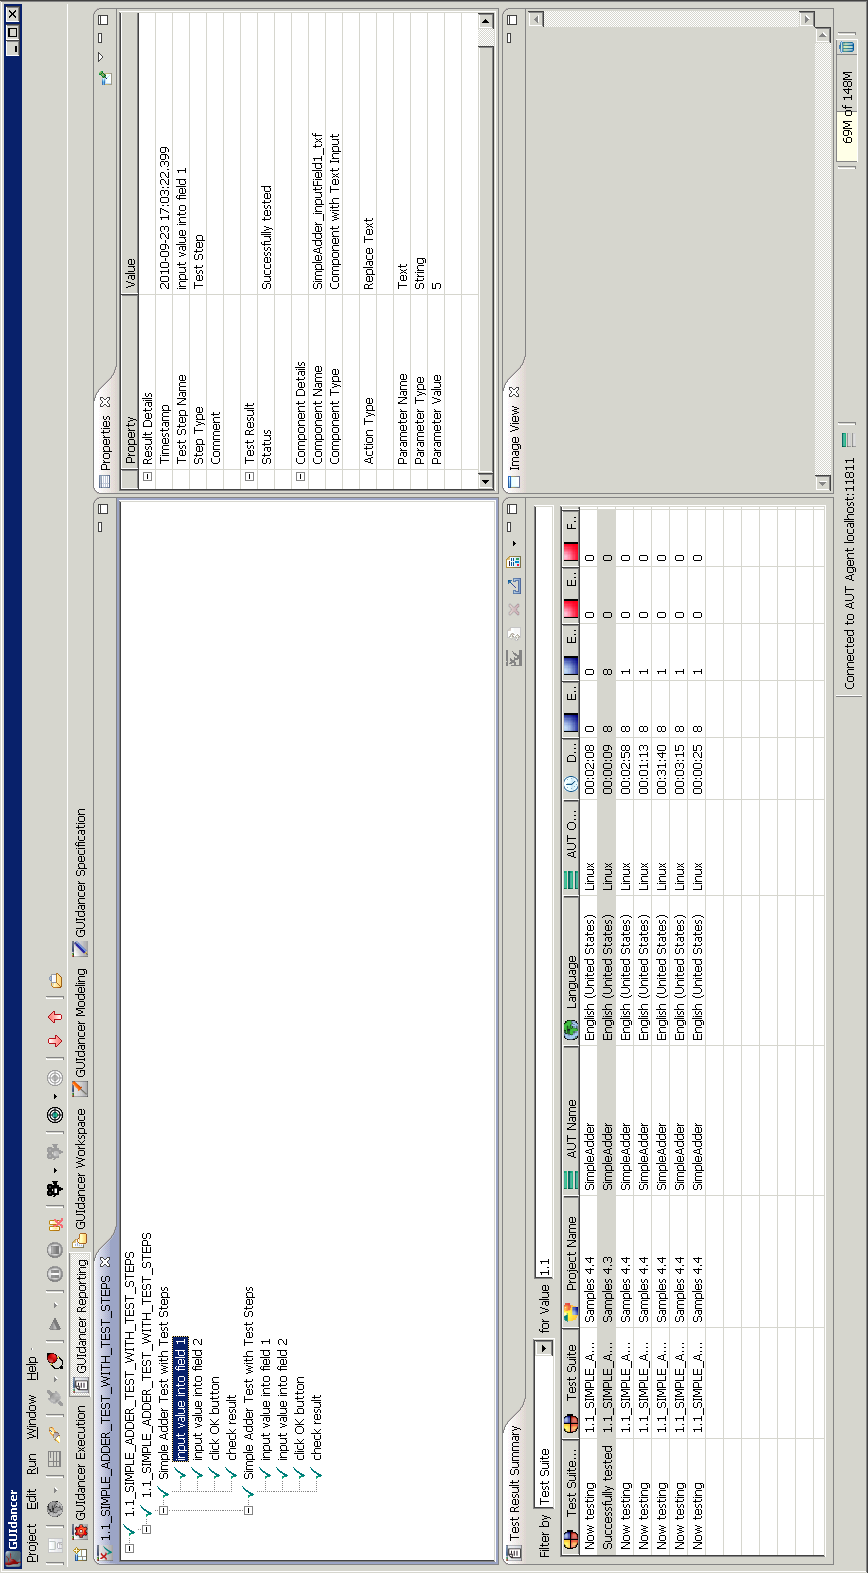
\includegraphics[width=12.5cm]{Userinterface/Editors/PS/reportingperspective}
\caption{\app{} Reporting Perspective}
\label{reportingperspective}
\end{figure}
\clearpage


\subsection{The \app{} workspace perspective}
\index{Perspective!Workspace}
\index{Workspace!Perspective}
\index{Views!Navigator}
\index{Navigator View}


In the workspace perspective (\bxfigref{workspaceperspective}), you can view the \gdprojects{} and files in your workspace. The workspace perspective contains the following:


\begin{itemize}
\item \gdnavview{} 
\item An editor area to view e.g. Excel and HTML files.
\end{itemize}

\begin{figure}
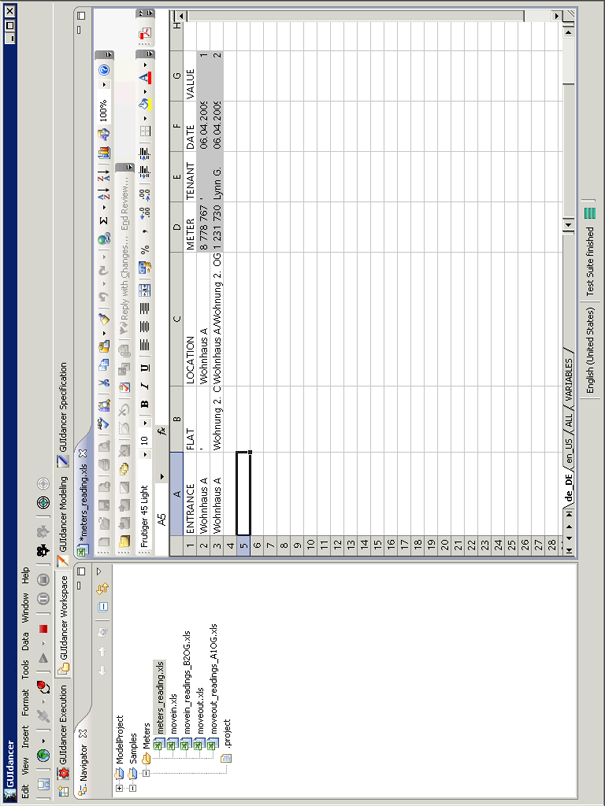
\includegraphics{Userinterface/Editors/PS/workspaceperspective}
\caption{\app{} Workspace Perspective}
\label{workspaceperspective}
\end{figure}
\clearpage


